\documentclass{deliverablereport}

\usepackage[style=alphabetic,backend=bibtex]{biblatex}
\addbibresource{report.bib}
\addbibresource{../../lib/publications.bib}

\usepackage{xparse}
\usepackage{etoolbox}
\usepackage{caption}
\graphicspath{{events/}}
 \ExplSyntaxOn

\newcounter{eventcounter}

\newenvironment{event}[7]{
\vspace{0.5cm}
\refstepcounter{eventcounter}
\label{event-#2}
\addcontentsline{toc}{subsection}{\hspace{3ex}-\ Event~\theeventcounter -~ #1}


\noindent\textbf{Event~\theeventcounter -~ #1}\newline % title

\noindent #3 \newline % location and date

\noindent ODK~partners~involved:~ \clist_map_inline:nn{#4}{\site{##1}~}\newline %partners

\ifx&#5&%
      % no participant #
\else
\noindent #5~participants~
\ifx&#6 &%
    % no odk participant
\else 
~(including~#6~from~within~ODK)\newline
\fi
\fi

\ifx&#7&%
      % no website
\else
\noindent \url{#7}\newline
\fi



}{\begin{center}\noindent\rule{4cm}{0.4pt}\end{center}}

 \ExplSyntaxOff


\deliverable{dissem}{workshops-4}
\duedate{31/08/2019 (M48)}
\deliverydate{31/08/2019}
\author{Viviane Pons et al.}

\begin{document}
\maketitle
\githubissuedescription
\newpage
\tableofcontents
\newpage

\section{Development workshops}

\TODO{EDIT}
We call a development workshop an event with a restricted number of participants
who meet to work on a specific task. These workshops are an inherent part
of \ODK development process as described in \taskref{dissem}{devel-workshops}:
 they bring together
developers from within and outside of \ODK and allow effective work
and discussions on many technical aspects. They also participate in building
and maintaining a community of developers inside \ODK and within the
open-source communities we belong to.

Throughout years 2 and 3 of the project, we have had 15 workshops dedicated mostly
to development. Some of them also included a training approach. 

\begin{event}{Atelier PARI/GP 2019}{AtelierPARI2019}{Bordeaux (FR),
2019-01-14 to 2019-01-18}{PS,UB,UV,UW}{36}{6}{http://pari.math.u-bordeaux.fr/Events/PARI2019/}


\textbf{\ODK implication.} \ODK participants: B. Allombert, K. Belabas, J.
Cremona, V. Delecroix, J.  Demeyer, L. de Feo.

\ODK provided the main funding source for the workshop (accommodation,
subsistence and some travel expenses), for about 13k\euro.

\textbf{Event summary.} The 12th Atelier PARI/GP took place in Bordeaux
(France) from january 14h to 18th.

There were 57 registered participants from 31 different institutions
(no registration fees).

A typical day of the workshop had introductory talks and tutorials
in the morning; afternoons allowed ample time for hacking sessions,
discussions and training.

The Atelier featured 10 morning talks on mathematical topics and
implementation projects including 4 talks by \ODK members
\begin{itemize}
\item Bill Allombert ``New GP features'' and ``Parallel GP programming''.
\item John Cremona ``Computing classical modular forms for the LMFDB''.
\item Jeroen Demeyer ``\texttt{cypari2}: Python bindings for PARI/GP''.
\end{itemize}

Slides for all talks are available at
\url{http://pari.math.u-bordeaux.fr/Events/PARI2019/}

\textbf{Results and impact.} The workshop was productive and a successful
teaching and dissemination event; 12 participants came from developping
countries (Algeria, Djibouti, Lebanon, Morroco, Senegal, Tunisia,
Turkey).

It provided final feedback on recent PARI/GP developments that paved the way
for the release of \texttt{pari-2.12-alpha} (2019/06).

\begin{figure}[ht]
  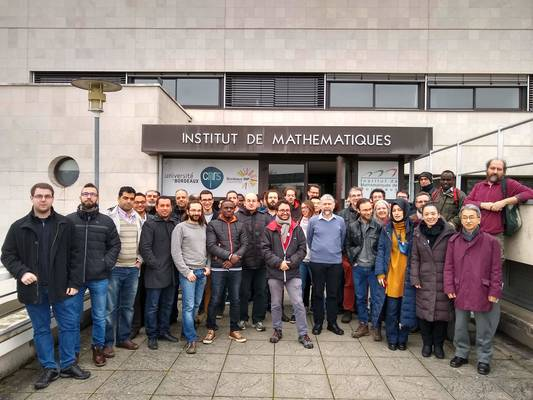
\includegraphics[width=.75\textwidth]{pari2019.jpg}
  \caption*{PARI/GP Atelier 2019, Bordeaux, France}
\end{figure}

\end{event}


\section{Dissemination and outreaching activities}

\TODO{EDIT}

We describe here all activities related to \taskref{dissem}{dissemination}:
these are all events oriented towards dissemination, training, and outreach. This
includes events organized or co-organized by \ODK and also
participating in external events and many communication activities.

\subsection{Training workshops and events}

\begin{event}{Software Tools for Mathematics}%
{STM_2018_09_Koper}{Koper, Slovenia, 2018-09-24--2018-09-28}%
{PS}{43}{3}{http://stm.famnit.upr.si/}

\textbf{Main goals.} The goal of the event was for mathematicians
to improve their coding skills and knowledge of mathematical software.

\textbf{ODK implication.} Samuel Lelièvre (\ODK member from UPSud) was one of
the organisers. The OpenDreamKit funds at Paris-Sud were used to fund travel
and stays of speakers.
The Faculty of Mathematics, Natural Sciences and Information Technologies at the University of Primorska
and Andrej Marušič Institute at the University of Primorska 
provided coffee and snacks at coffee breaks as well as equipped lecture rooms. 
The Slovenian Discrete and Applied Mathematics Society provided gifts for all participants.

\textbf{Event summary.} 
The event consisted in a two-day Software Carpentry
workshop (teaching participants the Unix shell, version control with Git,
and programming with Python) followed by three days on mathematical software
with mini-courses on CoCalc, GAP, SageMath and Jupyter, LaTeX and TikZ, as well
as talks on other mathematical software and databases, and on mathematical
research using software. A problem session allowed participants to submit
mathematical problems they cared about and thought software might help with,
a few of which were solved in the following days by other participants.

\textbf{Demographic.} 
The participants included a small number of bachelor students,
several PhD students and postdocs, professors and researchers.

\textbf{Results and impact.}

At the Software Carpentry workshop, 
the Unix shell was taught by Peter Palfrader and Jan Ber\v{c}i\v{c}, 
Git was taught by Alexander Konovalov and Peter Palfrader,
and Python was taught by Julian R\"{u}th and Nino Ba\v{s}i\'{c}.

During the mathematical software part,
Alexander Konovalov taught GAP,
Nino Ba\v{s}i\'{c} taught LaTeX and TikZ,
Samuel Leli\`{e}vre taught SageMath and CoCalc,
and Julian R\"{u}th taught SageMath.

Many participants told the organisers, orally or by email, that this workshop
was transformative for them; often they felt they had passed some confidence
threshold: whereas before the conference they were interested in mathematical
software but unsure how to install and use them, they were now confident how
to do that, and felt they had the necessary resources to learn more.
One of the participants even commented that they were able to use what they learned
immediately in their research.
Some of the participants are involved in the organisation of the upcoming 
European Congress of Mathematics (ECM 2020 Portoro\v{z}, Slovenia),
and expressed interest in highlighting open software for mathematics at the ECM.

Furthermore, a CoCalc instance was installed on University of Primorska servers
due largely to this event.

This event was conceived due to the success of the Software Tools for Mathematics
in Morelia earlier in 2018.
Based on the success of both workshops,
Samuel Leli\`{e}vre and Katja Ber\v{c}i\v{c} (who participated in the organisation of both)
hope that the series will continue and are considering options for future installments.

\begin{figure}[ht]
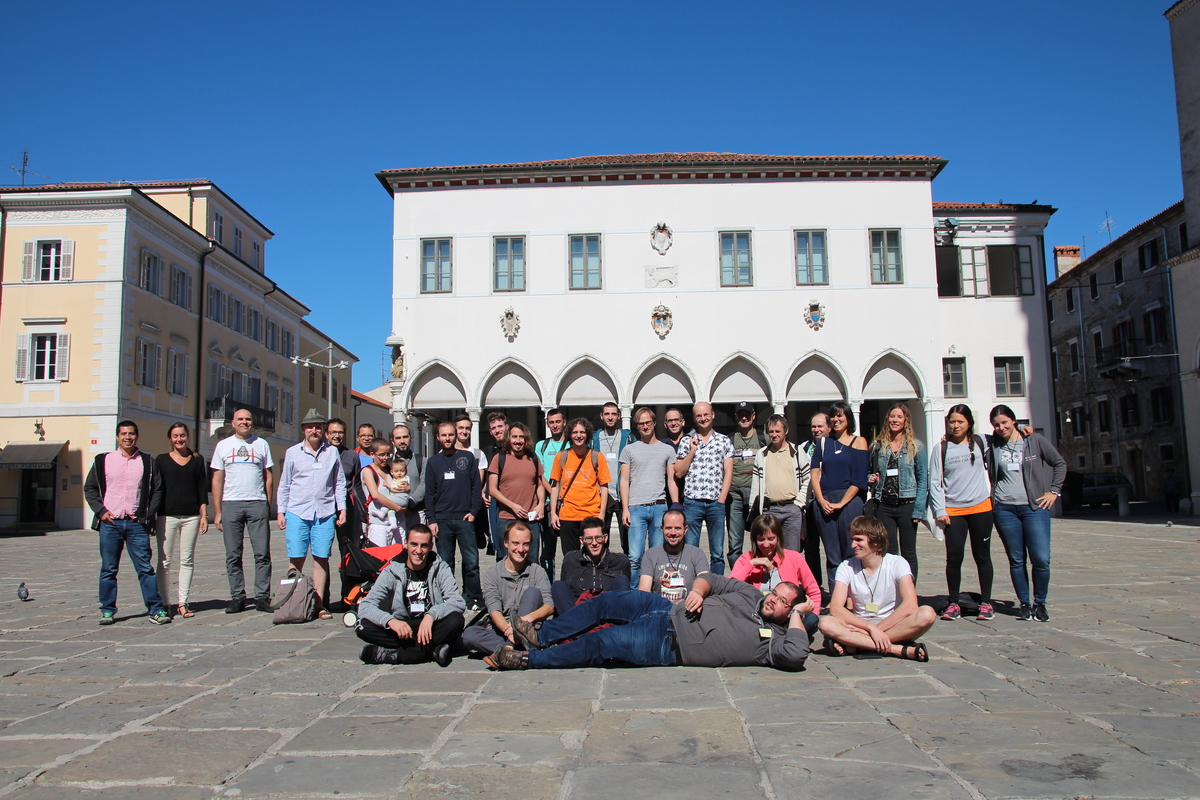
\includegraphics[scale=0.3]{stm-koper2019.jpeg}
\caption*{Software Tools for Mathematics in Koper, Slovenia}
\end{figure}



\end{event}



\begin{event}{SageMath classes in Crete}{crete}{Heraklion, March. 4-6, 2019}{PS}{10}{1}{}

\textbf{Main goals.} We organized a series of SageMath classes in the mathematical department of the Univeristy of Crete.

\textbf{ODK implication.} OpenDreamKit funded the trip of Viviane Pons to give the classes.

\textbf{Event summary.} A series of three classes was organized throughout the week. This was open both to students (from undergrad to PhD) and researchers of the math department of the Univeristy of Crete. The classes consisted of SageMath tutorials to allow the attendees to discover the software at their own pace. We used Jupyter notebooks with a focus on math related problems.

\textbf{Results and impact.} The students enjoyed the tutorials a lot. It was actually used as a starting point for more regular sessions tutored by their local teacher Eleni Tzanaki. We are now confident that SageMath will be taught at Univeristy of Crete as part of the math program.  The meeting was also an occasion to prepare the up-coming Women in Sage event also organized in Crete. 

\end{event}

\begin{event}{Atelier PARI/GP 2019b}{AtelierPARI2019b}{Roma (IT),
2018-04-09 to 2018-04-10}{UB}{36}{6}{http://pari.math.u-bordeaux.fr/Events/PARI2019b/}

\textbf{Main goals.} This was a teaching and dissemination meeting, by
invitation from the Roman Number Theory Association as a satellite
event for their 5th mini-symposium.

\textbf{\ODK implication.} \ODK participants: B. Allombert and A. Page from
Bordeaux.

\ODK funded travel and accomodation costs for B. Allombert for about
  1.5k\euro. The ALGANT consortium, LIA LYSM (CNRS) and University Roma Tre
  co-funded the event.

\textbf{Event summary.} This Atelier PARI/GP took place in Roma (Italy) on
April 9th and 10th.  It was followed by a 3-day international research
conference on Number Theory. There were 40 participants for the
Atelier.

The 2-day Atelier followed the same pattern as the previous Roma Atelier
in 2018,
featuring a general introduction to PARI/GP and two
  specialized courses (graduate level) in the mornings:
\begin{itemize}
\item Bill Allombert ``Finite fields'',
\item Aurel Page ``Algebraic number theory''.
\end{itemize}
Afternoons were devoted to practice and problem sessions.

Slides for all talks are available at
\url{http://pari.math.u-bordeaux.fr/Events/PARI2019b/}

\textbf{Results and impact.} This was a successful teaching and dissemination
event, with positive feedback from the participants and organizers.

\begin{figure}[ht]
  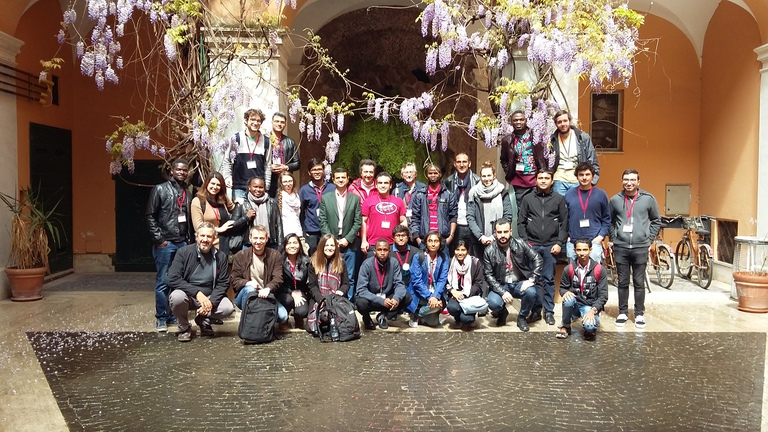
\includegraphics[width=.75\textwidth]{pari2019b.jpg}
  \caption*{Atelier PARI/GP, 5th Roman Number Theory Association mini-symposium, Rome}
\end{figure}
\end{event}




\subsection{Organization of Sage Days in established mathematical communities}

One goal of \ODK is to support local communities of researchers
and developers who contribute to the open-source software related to
the project. For \Sage, this means supporting the organization of Sage-Days
workshops that arise from within all the different mathematical communities. The main 
goal of these workshops is mostly to improve the Sage coverage of some mathematical
area. They also play a major role in training and communication. The
impact for \ODK can be summarized this way:

\begin{itemize}
\item \textbf{Making \ODK known to the end users}: by supporting Sage Days,
\ODK makes itself known to the Sage community and can
thus share the many developments of the project.

\item \textbf{Improving the overall quality of Sage}: by fostering researchers
in specific areas, Sage Days help bring interesting mathematics into
the software, which is beneficial for Sage and so \ODK.

\item \textbf{Training, bringing more user}: Sage Days are the perfect place
for new comers, especially students, to get their first experience with the software.

\item \textbf{Fostering a community}: Sage Days are helping making Sage a vibrant
community, which is vital for the success of \ODK.
\end{itemize}



\subsection{Training activities in developing countries}


\subsection{Women in \ODK}

\TODO{EDIT}
\ODK is aware of the gender gap that exists in science in general
and more specifically in software development. We have been organizing
events to support specifically women developers, engineers and scientists.

\begin{event}{Sage Days 98 : Women in Sage}{SD98}{Archanes (Greece), April 8 -- April 12, 2019}{PS}{22}{1}{https://opendreamkit.org/2019/06/28/WomenInSage/}

\textbf{Main goals.} The main goal of the event was to initiate more women to the software \Sage to reduce the gender gap in mathematics software
development. Each participant had to propose a mathematic development project to be carried out during the week.

\textbf{\ODK implication.} The event was initiated by Viviane Pons from \ODK and co-organized with Eleni Tzanaki (University of Crete). It was funded solely by \ODK which covered: lodging for the participants (rented houses), food, and transportation for many of the participants.

\textbf{Event summary.} The event was organized as a workshop where every participant could work on their own project to develop their coding skills. We started the week with an introduction to Sage and some tutorials. Then each participant gave a 5 minute talk about their own research. After that, we worked on different projects, organizing status reports every day. In particular, we ran a group specifically to produce new contributions to Sage.

\textbf{Demographics.} All participants were women coming from 8 different countries (France, Belgium, Germany, Greece, UK, US, Romania and Peru), as per institutions, and more if we count nationalities (Australia, Lebanon, Spain). About half of them could be considered Sage beginners. We had 1 master student, 14 PhD students, 2 postdocs, and 5 \textit{Maîtresses de conférences} or assistant professor or lecturer.

We were supposed to also welcome 3 women from Nigeria but they were sadly not able to obtain their visas on time.

\textbf{Results and impact.} A full report on the impact of this
workshop can be read on our website:
\centerline{\url{https://opendreamkit.org/2019/06/28/WomenInSage/}}
The main goal was to make the participants more confident into their programming skills and more prone to become Sage contributors and attend classical Sage Days. It was a big success in that regard. Indeed, before the conference, only 17\% of the participants had attended Sage Days more than once and 50\% had never heard of it. After, the conference, 94\% rated 3 or more out of 5 the chances that they would attend Sage Days event in the future. 100\% of the participant rated 3 or more out of 5 the impact of the workshop on their future career and 100\% said they met interesting people. Additionally, work was done on 5 Sage issues from of which 3 have been merged into Sage source code already.

\begin{figure}[ht]
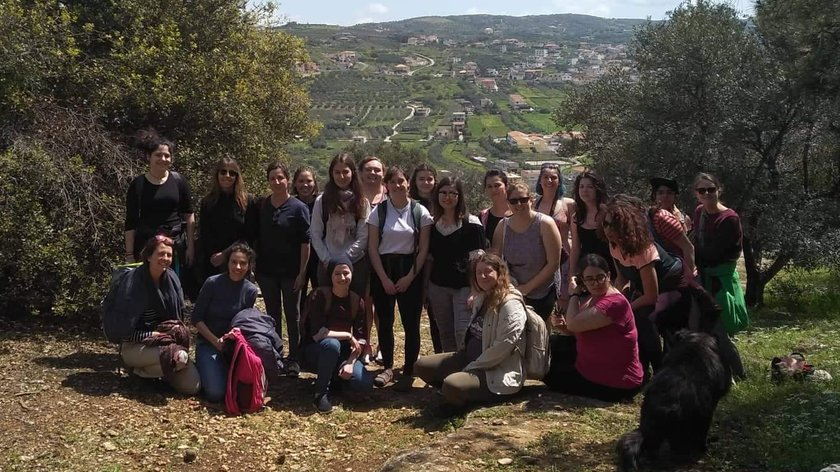
\includegraphics[scale=.3]{group_photo_head.jpeg}
\caption*{Women in Sage in Archanes}
\end{figure}



\end{event}


\subsection{Organization of research workshopts}

\begin{event}{Journées Nationales de Calcul Formel}{JNCF2019}{Luminy (FR),
  2019-02-04 to
  2019-02-08}{UV,UJF}{58}{3}{http://www.jncf2019.uvsq.fr/}
  
\textbf{Main goals.} This is the yearly meeting of the French community in
Computer Algebra, open to an international audience, with lectures and
contributed talks given mostly in English.

\textbf{\ODK implication.} Luca De Feo co-organized the JNCF 2019. The
organization of the workshop was coordinated with the organization of
the ``Free Computational Mathematics'' conference, taking place the
following week in the same venue, to encourage cross-participation.

Luca De Feo and Clément Pernet gave presentations on Monday on the
achievements of \ODK relevant to the Computer Algebra
community.

\ODK participants: Luca De Feo from University of Versailles,
Jean-Guillaume Dumas and Clément Pernet from University Grenobles
Alpes.

\ODK sponsored the event (3000\euro \TODO{Double-check the figure}).

\textbf{Event summary.} This conference took place in Luminy (France) from
February 4th to 8th. About 58 mathematicians and computer scientists
participated to the event. Three of the participants also participated
in the ``Free Computational Mathematics'' conference the following
week, while four other noted members of the French community in
Computer Algebra, Joris van der Hoeven, Marie Françoise Roy, Fredrik
Johansson and Bill Allombert, elected to only participate in the latter
due to time constraints.

Slides for Luca De Feo and Clément Pernet's presentations are
available online from the conference web page:
\url{http://www.jncf2019.uvsq.fr/edt.html}.

\textbf{Results and impact.} Computer Algebra is the birth place of
computer-aided Mathematics, and all of \ODK software owe something to
the field. Over the years, \ODK has constantly used the JNCF as an
occasion to disseminate its achievements relevant to the community,
through contributed talks.

The last edition of JNCF to happen concomitantly with the project was
the occasion to double the dissemination efforts, and organize the
JNCF in tandem with the main \ODK conference ``Free Computational
Mathematics'': two invited talks at the ``Free Computational
Mathematics'' were delivered by noted members of the French Computer
Algebra community, while one of the invited lectures at JNCF was
delivered by Mohamed Barakat, a GAP developer and founder of the OSCAR
consortium, close to the \ODK community. A full session was devoted to
mathematical software on Monday afternoon, with two presentations
given by \ODK members, and one by a MapleSoft executive, which
triggered visible interest in the audience.

This was a successful workshop, and a great occasion to deliver 
successful developments of \ODK to its user base.
\end{event}


\subsection{Communication and participation to external events}

\begin{event}{Keynote at PyconFr}{pyconfr}{Lille (France), Oct. 6, 2018}{PS}{400}{1}{https://www.pycon.fr/2018/}

\textbf{Main goals.} PyConFr is the annual gathering of the French python community. 

\textbf{ODK implication.} Viviane Pons was invited to be the opening keynote of the conference.

\textbf{Event summary.} She gave a 30 minutes talk on ``Science and Open-Source: what do we learn from each other'' This was an occasion to discuss the many interactions between research and open-source development and highlight the role of projects such as OpenDreamKit.

\textbf{Results and impact.} The talk was well received by the python community with many positive feedbacks.

\end{event}

\begin{event}{CIRM2019: Conference Cohomology of arithmetic groups, lattice and number
  theory, in Luminy}{CIRM2019}{Luminy (FR),
  2019-03-24 to
  2019-03-29}{UB}{36}{6}{https://conferences.cirm-math.fr/1995.html}
  
\textbf{Main goals.} This was a research conference on the cohomology of
arithmetic groups, with a focus on computational techniques.

\textbf{\ODK implication.} Bill Allombert was invited to give a 1-hour
introduction to PARI/GP for a software session during the conference.
He gave a tutorial on the manipulation of lattices, $L$-functions,
modular forms and curves of small genus in the system.

\ODK participants: B. Allombert from Bordeaux.

\ODK funded the participation of B. Allombert to the event (about 600\euro).

\textbf{Event summary.} This conference took place in Luminy (France)
from March 24th to 29th, with the participation of about 70 mathematicians.

Slides for the PARI/GP presentation are available at
\url{http://pari.math.u-bordeaux.fr/Events/CIRM2019/}

\textbf{Results and impact.} This was a successful teaching and dissemination
event towards a community (arithmetic geometry, representation theory)
for which computer-aided calculations is less natural than in other
areas of mathematics: the talk was well-received with interesting
feedback.
\end{event}


%\newpage\printbibliography

\end{document}

%%% Local Variables:
%%% mode: latex
%%% TeX-master: t
%%% End:
